%	Este arquivo não esta oroginalmente incluso e representa apenas um
%	breve modelo de como se produzir uma capa personalizada

\begin{titlepage}

\centering
\hfill
\includegraphics[keepaspectratio,scale=0.05]{images/unb.png}%
\hfill
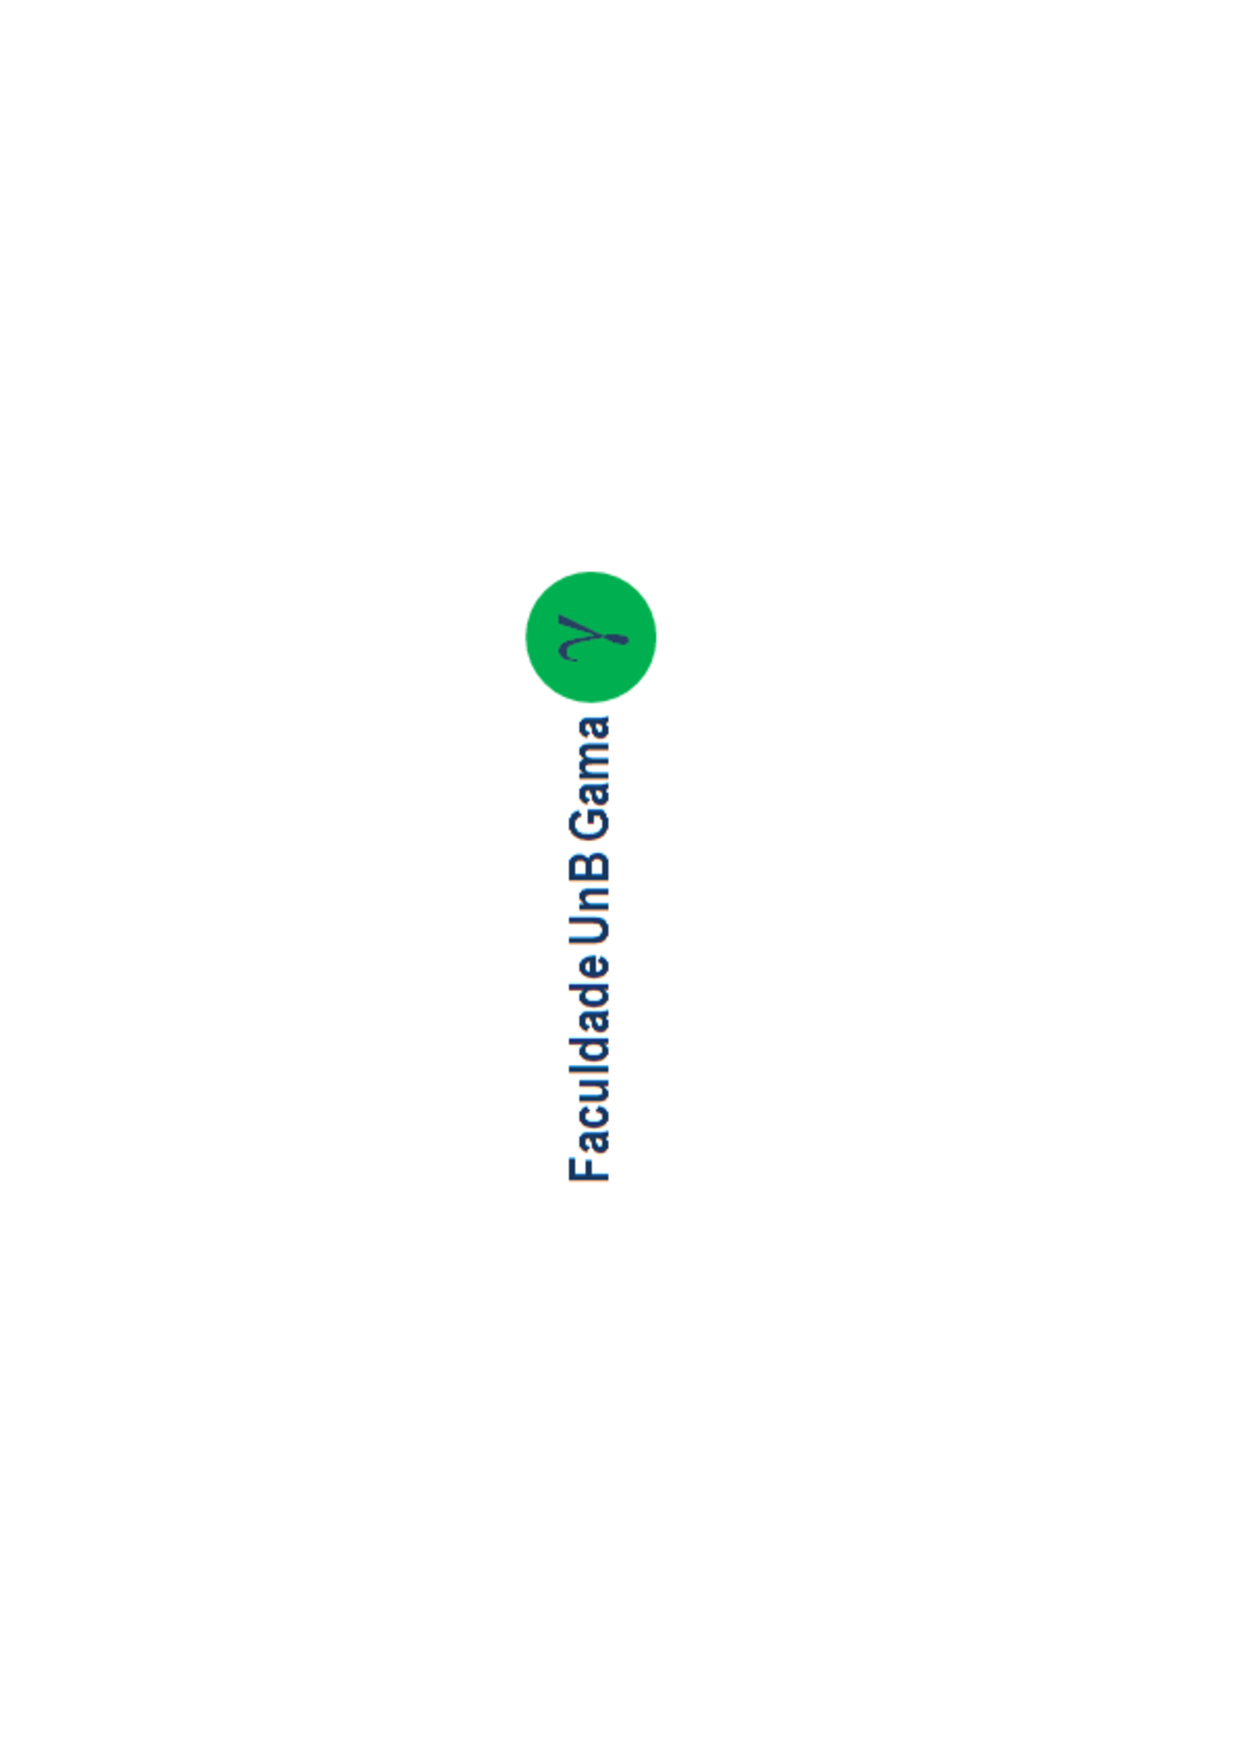
\includegraphics[keepaspectratio,scale=0.5]{images/fga.png}
\hfill

% \doublespacing
\scshape
\normalfont
\vspace{2cm}

\vspace*{\fill}

%Nome do Trabalho

\huge{\ver}

\vspace{0.03\textheight}
% \hrule
\vspace{0.01\textheight}

%Nome da Materia
{\Huge{\hell}}


\vspace*{\fill}

\vspace{0.3\textheight}
%Nomes
\vbox{\scshape
	\vbox{\large Universidade de Brasília - UnB\\Faculdade Gama – FGA}
}
\vspace{0.25cm}
\vbox{\normalsize Brasília, DF – \today}
\end{titlepage}
